\documentclass[12pt,a4paper]{article}
\usepackage[utf8]{inputenc}
\usepackage[spanish,es-nodecimaldot,es-tabla]{babel}
\usepackage{graphicx}
\usepackage{float}
\usepackage{geometry}
\usepackage{hyperref}
\usepackage{fancyhdr}
\usepackage{titlesec}
\usepackage{booktabs}
\usepackage{xcolor}
\usepackage{verbatim}
\usepackage{mathptmx}
\usepackage{setspace}
\usepackage{xurl}
\usepackage{amsmath}

\geometry{top=2.5cm, bottom=2.5cm, left=3cm, right=3cm}
\hypersetup{colorlinks=true, linkcolor=black, urlcolor=blue, citecolor=black}
\graphicspath{{../resultados/figuras/}{figuras_codigo/}}

\pagestyle{fancy}
\fancyhf{}
\fancyhead[L]{\small Búsqueda local en el 8-puzzle}
\fancyhead[R]{\thepage}
\renewcommand{\headrulewidth}{0.4pt}
\setlength{\headheight}{15pt}

\titleformat{\section}{\normalfont\Large\bfseries}{\thesection}{1em}{}
\titleformat{\subsection}{\normalfont\large\bfseries}{\thesubsection}{1em}{}
\titleformat{\subsubsection}{\normalfont\normalsize\bfseries}{\thesubsubsection}{1em}{}

\begin{document}

\begin{titlepage}
\thispagestyle{empty}
\centering

\vspace*{0.5cm}

\includegraphics[width=0.30\textwidth]{sergio_logo.png}\\[0.4cm]

{\fontsize{13}{15}\selectfont\textbf{UNIVERSIDAD SERGIO ARBOLEDA}}\\[2.5cm]

{\fontsize{14}{17}\selectfont\textbf{BÚSQUEDA LOCAL EN EL 8-PUZZLE:\\[0.2cm]
ASCENSO DE COLINAS Y TEMPLE SIMULADO}}\\[3.5cm]

{\fontsize{12}{14}\selectfont\textbf{Introducción a la Inteligencia Artificial}}\\[1.8cm]

{\fontsize{12}{14}\selectfont Mario Jiménez}\\[0.3cm]
{\fontsize{12}{14}\selectfont Juan David Andrade}\\[0.3cm]
{\fontsize{12}{14}\selectfont Camilo Andrés Díaz García}\\[0.3cm]

\vfill

\begin{center}
    \textit{Universidad Sergio Arboleda}\\
    \textit{Facultad de Sistemas e Ingeniería}\\
    \textit{Bogotá D.C., 2026}
\end{center}

\end{titlepage}

\newpage
\tableofcontents
\newpage

\onehalfspacing

% ====================================================================
\section{Introducción}

Este taller aplica búsqueda local al 8-puzzle y compara dos familias
de algoritmos: el ascenso de colinas, en tres variantes (más
pronunciado, estocástico y con reinicios), y el temple simulado. El
objetivo no es solo reportar cuál resuelve más tableros, sino mostrar
con evidencia cómo se adapta cada algoritmo a la estructura del
problema y qué decisiones de diseño hicieron falta para que la
comparación fuera justa.

Todos los algoritmos se evaluaron sobre el mismo conjunto de 30
tableros resolubles, con el mismo presupuesto de evaluaciones de la
función objetivo y con 10 semillas aleatorias por tablero. Los
parámetros de temple simulado se eligieron con un barrido
sistemático, y el largo de la perturbación de los reinicios se fijó
con un criterio derivado del diámetro del espacio de estados. Además
de la tasa de éxito se midió el costo (evaluaciones de $h$) y la
calidad de la solución encontrada (número de movimientos frente a la
solución óptima de cada tablero).

Este documento presenta el marco teórico, la metodología y el análisis
de los resultados. La implementación completa, los experimentos
reproducibles y las tablas y figuras junto al código que las genera
están en el cuaderno adjunto (\nolinkurl{taller_8puzzle.ipynb}) y en el
repositorio del equipo
(\url{https://github.com/CamiloDG07/Taller_Colina-Temple}). Los
fragmentos de código que aparecen aquí son capturas generadas
directamente desde ese código fuente, así que sus números de línea
coinciden con los de los archivos.

% ====================================================================
\section{Marco teórico}

\subsection{Búsqueda local}

Los algoritmos de búsqueda clásicos (anchura, profundidad, A*) exploran
el espacio de estados de forma sistemática y guardan en memoria los
caminos desde el estado inicial. La búsqueda local sigue otra idea:
mantiene uno o pocos estados actuales y se mueve solo a estados
vecinos, sin recordar los caminos recorridos \cite{russell2021}. Tiene
dos ventajas: usa muy poca memoria (constante, en la práctica) y puede
encontrar soluciones razonables en espacios enormes o continuos donde
una búsqueda sistemática no es viable.

La búsqueda local trabaja con una \emph{formulación de estado completo}:
cada estado es una configuración completa del problema y el algoritmo
la va modificando. La calidad de un estado se mide con una función
objetivo; en este taller se minimiza una función de costo $h(s)$, cuyo
mínimo global ($h = 0$) corresponde a la meta.

\subsubsection{El paisaje del espacio de estados}

Es útil imaginar el espacio de estados como un paisaje, donde la
posición es el estado y la altura es el valor de $h$. Un algoritmo de
minimización busca el valle más profundo. Las dificultades clásicas
son \cite{russell2021}:

\begin{itemize}
    \item \textbf{Mínimos locales}: estados en los que todos los vecinos
    tienen $h$ mayor o igual, pero que no son el mínimo global. Un
    algoritmo que solo acepta mejoras queda atrapado en ellos.
    \item \textbf{Mesetas}: regiones donde los vecinos tienen el mismo
    valor de $h$, sin gradiente que indique hacia dónde avanzar.
    \item \textbf{Crestas}: secuencias de mínimos locales que exigen
    una combinación de movimientos, y no uno solo, para mejorar.
\end{itemize}

Un algoritmo de búsqueda local es \emph{completo} si siempre encuentra
una meta cuando existe, y \emph{óptimo} si encuentra el mínimo global.
Un algoritmo que nunca acepta empeorar es incompleto: puede quedar
atrapado en un mínimo local. Un paseo puramente aleatorio es completo
en un espacio finito, pero extremadamente ineficiente. Los algoritmos
de este taller combinan de distintas formas la explotación (moverse
hacia menor $h$) y la exploración (aceptar movimientos que no mejoran).

\subsection{Formulación del 8-puzzle}

El 8-puzzle es un tablero de $3 \times 3$ con ocho fichas numeradas y
una casilla vacía. Un movimiento desliza una ficha adyacente a la
casilla vacía hacia ella. La meta es el tablero ordenado
$(1, 2, 3, 4, 5, 6, 7, 8, \text{vacía})$.

\begin{itemize}
    \item \textbf{Estado}: una tupla de 9 valores con la posición de
    cada ficha (0 representa la casilla vacía).
    \item \textbf{Vecindad}: los estados que se obtienen con un
    movimiento legal de la casilla vacía (arriba, abajo, izquierda o
    derecha). Cada estado tiene entre 2 y 4 vecinos según la posición
    de la casilla vacía (esquina, borde o centro).
    \item \textbf{Función objetivo}: la distancia Manhattan,
    \begin{equation}
        h(s) = \sum_{i=1}^{8} \left( |f_i(s) - f_i^*| + |c_i(s) - c_i^*| \right),
    \end{equation}
    donde $(f_i(s), c_i(s))$ es la posición de la ficha $i$ en el
    estado $s$ y $(f_i^*, c_i^*)$ su posición en la meta. Se cumple
    $h(s) = 0$ si y solo si $s$ es la meta.
\end{itemize}

La Figura \ref{fig:codigo_manhattan} muestra la implementación de la
función objetivo. Recorre las nueve casillas, salta la vacía (líneas
38 y 39) y suma la distancia horizontal y vertical de cada ficha a su
posición en la meta (líneas 40 a 43). Como cada término es no
negativo y solo vale 0 cuando la ficha ya está en su lugar, $h(s) = 0$
únicamente en la meta. Eso permite usar la misma condición, $h = 0$,
como criterio de éxito en todos los algoritmos.

\begin{figure}[H]
    \centering
    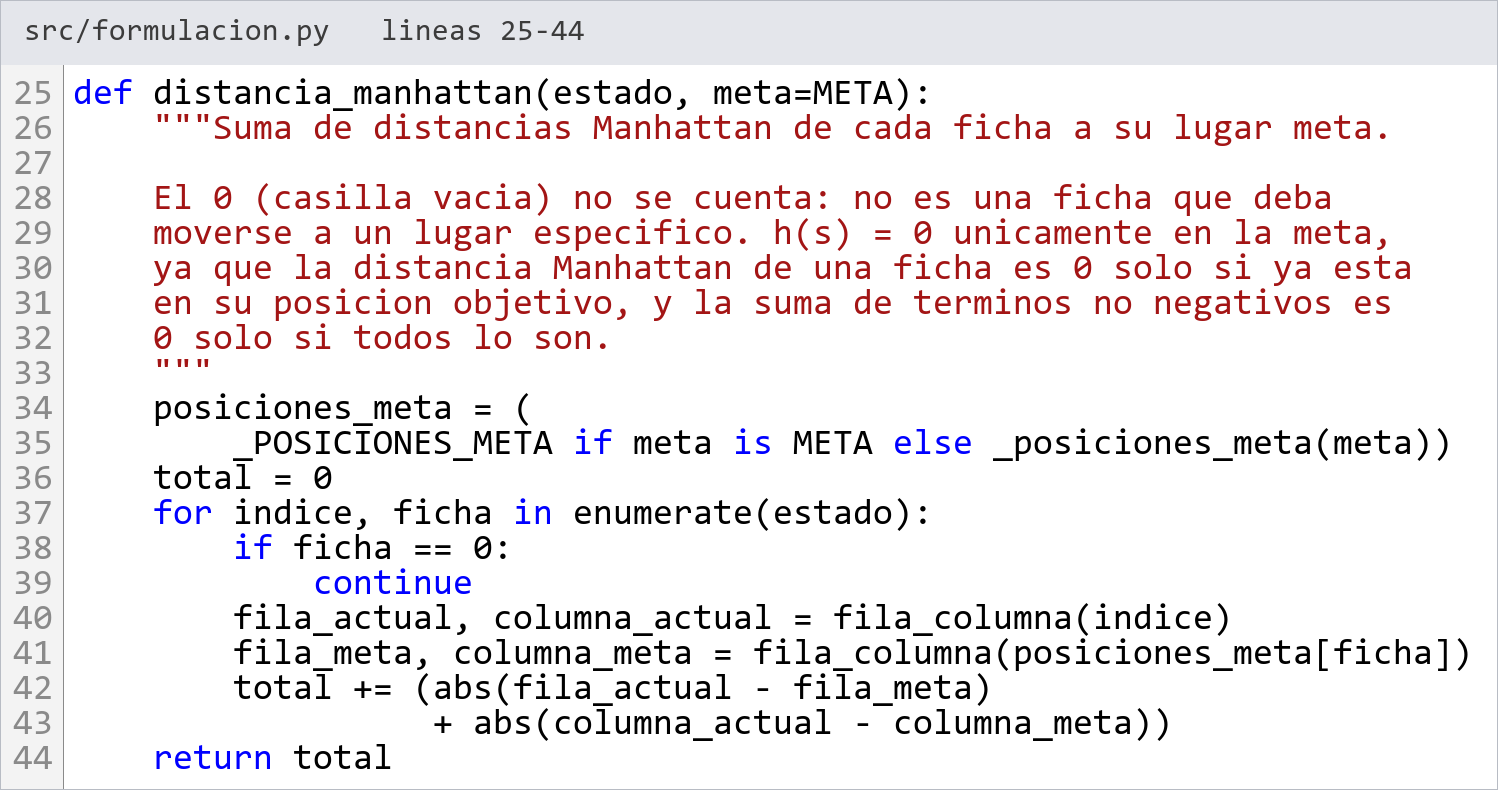
\includegraphics{distancia_manhattan.png}
    \caption{Función objetivo $h(s)$: distancia Manhattan. Fuente:
    elaboración propia (\nolinkurl{src/formulacion.py}).}
    \label{fig:codigo_manhattan}
\end{figure}

Dos propiedades de esta formulación son importantes para el análisis:

\begin{enumerate}
    \item \textbf{Cada movimiento cambia $h$ exactamente en $\pm 1$}:
    un movimiento desplaza una sola ficha una casilla, y esa ficha se
    acerca o se aleja de su destino en una unidad. Por eso no hay
    movimientos laterales ($\Delta h = 0$) ni mesetas en sentido
    estricto. Esta propiedad se verificó en el código
    (\texttt{verificar\_delta\_h}).
    \item \textbf{Solo la mitad de los tableros es resoluble}: de los
    $9! = 362\,880$ tableros posibles, solo $9!/2 = 181\,440$ pueden
    llegar a la meta. Un tablero es resoluble si su número de
    inversiones (pares de fichas en orden inverso, sin contar la
    casilla vacía) es par \cite{johnson1879}. El generador de tableros
    de prueba solo produce tableros resolubles.
\end{enumerate}

Además, la solución óptima de cualquier tablero resoluble tiene como
máximo 31 movimientos: ese es el \emph{diámetro} del espacio de estados
\cite{reinefeld1993}. Este dato se verificó en este trabajo con una
búsqueda en anchura desde la meta sobre los 181\,440 estados
resolubles: la distancia máxima encontrada fue exactamente 31. La misma
búsqueda da la longitud óptima de cada tablero de prueba, que se usa
para medir la calidad de las soluciones.

\subsection{Ascenso de colinas}

El ascenso de colinas (\emph{hill climbing}) es la búsqueda local más
simple: en cada paso se mueve a un vecino que mejora la función
objetivo y se detiene cuando ninguno la mejora \cite{russell2021}. Es
un algoritmo voraz: toma la mejor decisión local sin considerar
consecuencias futuras.

\begin{itemize}
    \item \textbf{Más pronunciado} (\emph{steepest ascent}): evalúa
    todos los vecinos y se mueve al de menor $h$. Es determinista.
    \item \textbf{Estocástico}: evalúa todos los vecinos y elige al
    azar entre los que mejoran $h$. Suele avanzar más despacio, pero a
    veces encuentra mejores soluciones en paisajes con muchas
    direcciones de mejora.
    \item \textbf{Con reinicios aleatorios} (\emph{random restart}):
    repite el ascenso desde distintos puntos de partida hasta encontrar
    la meta o agotar un presupuesto. Si cada intento tiene probabilidad
    $p$ de éxito, el número esperado de intentos es $1/p$, y el
    algoritmo es completo con probabilidad que tiende a 1
    \cite{russell2021}.
\end{itemize}

Las dos primeras variantes se detienen en el primer mínimo local. En
el 8-puzzle, como $\Delta h = \pm 1$, un paso de ascenso siempre baja
$h$ en exactamente 1, así que el camino de un ascenso tiene como máximo
$h(s_0)$ movimientos y nunca retrocede.

\subsection{Temple simulado}

El temple simulado (\emph{simulated annealing}) se inspira en el
recocido de metales: un material calentado y enfriado lentamente
alcanza una estructura cristalina de baja energía
\cite{kirkpatrick1983}. El algoritmo trata $h(s)$ como la energía del
estado. En cada iteración elige un vecino al azar y calcula
$\Delta E = h(s') - h(s)$:

\begin{itemize}
    \item si $\Delta E \le 0$ (el vecino no empeora), lo acepta siempre;
    \item si $\Delta E > 0$ (el vecino empeora), lo acepta con
    probabilidad
    \begin{equation}
        P(\text{aceptar}) = e^{-\Delta E / T},
    \end{equation}
    que es el criterio de Metropolis \cite{metropolis1953}.
\end{itemize}

La temperatura $T$ controla el equilibrio entre exploración y
explotación. Con $T$ alta casi todo empeoramiento se acepta y el
algoritmo se comporta como un paseo aleatorio. Con $T$ cercana a 0 casi
ningún empeoramiento se acepta y el algoritmo se vuelve un ascenso de
colinas. En el 8-puzzle, como $\Delta E = +1$ en todo empeoramiento, la
probabilidad de aceptarlo depende solo de $T$: vale $e^{-1} \approx
0.37$ con $T = 1$, $e^{-2} \approx 0.14$ con $T = 0.5$ y $e^{-20}$
(prácticamente cero) con $T = 0.05$.

Este trabajo usa enfriamiento geométrico: se hacen $L$ iteraciones con
cada temperatura y después se actualiza $T_{k+1} = \alpha \, T_k$,
desde $T_0$ hasta $T \le T_{\min}$. La ejecución también se detiene si
$h$ llega a 0. Los parámetros son la temperatura inicial $T_0$, el
factor de enfriamiento $\alpha \in (0, 1)$, las iteraciones por nivel
$L$ y la temperatura mínima $T_{\min}$. El número de niveles de
temperatura es
\begin{equation}
    N = \left\lceil \frac{\ln (T_{\min}/T_0)}{\ln \alpha} \right\rceil,
\end{equation}
y el costo máximo de una corrida es de unas $N \cdot L$ evaluaciones.
Existe un resultado teórico que garantiza la convergencia al óptimo
global con un enfriamiento logarítmico suficientemente lento
\cite{russell2021}, pero ese ritmo es impracticable. En la práctica,
elegir $T_0$ y $\alpha$ es un compromiso entre calidad y costo.

A diferencia del ascenso de colinas, el estado actual del temple puede
empeorar; por eso la implementación guarda aparte el mejor estado
visto, que nunca empeora. El temple no tiene memoria de los estados
visitados: puede aceptar un movimiento que deshace el anterior y volver
a zonas ya exploradas.

La Figura \ref{fig:codigo_temple} muestra el núcleo de la
implementación: una iteración de temple con la temperatura actual. Las
líneas 72 a 77 son el criterio de Metropolis. Si el vecino no empeora
($\Delta E \le 0$) se acepta siempre (líneas 73 y 74); si empeora, se
acepta solo cuando un número aleatorio uniforme cae por debajo de
$e^{-\Delta E / T}$ (líneas 76 y 77). Esa rama es la que permite al
temple salir de un mínimo local, y es exactamente lo que le falta al
ascenso de colinas. Otros tres detalles del fragmento sostienen
decisiones posteriores:

\begin{itemize}
    \item cada vecino evaluado suma una evaluación (líneas 69 y 70), el
    mismo criterio de costo que en el ascenso de colinas;
    \item el mejor estado se guarda aparte y solo cambia cuando mejora
    (líneas 82 y 83), así que el resultado final nunca empeora aunque
    el estado actual sí lo haga;
    \item \texttt{movimientos\_aceptados} cuenta todos los movimientos
    aceptados, incluidos los que empeoran $h$ (línea 81); por eso la
    longitud de la solución del temple incluye su zigzagueo.
\end{itemize}

\begin{figure}[H]
    \centering
    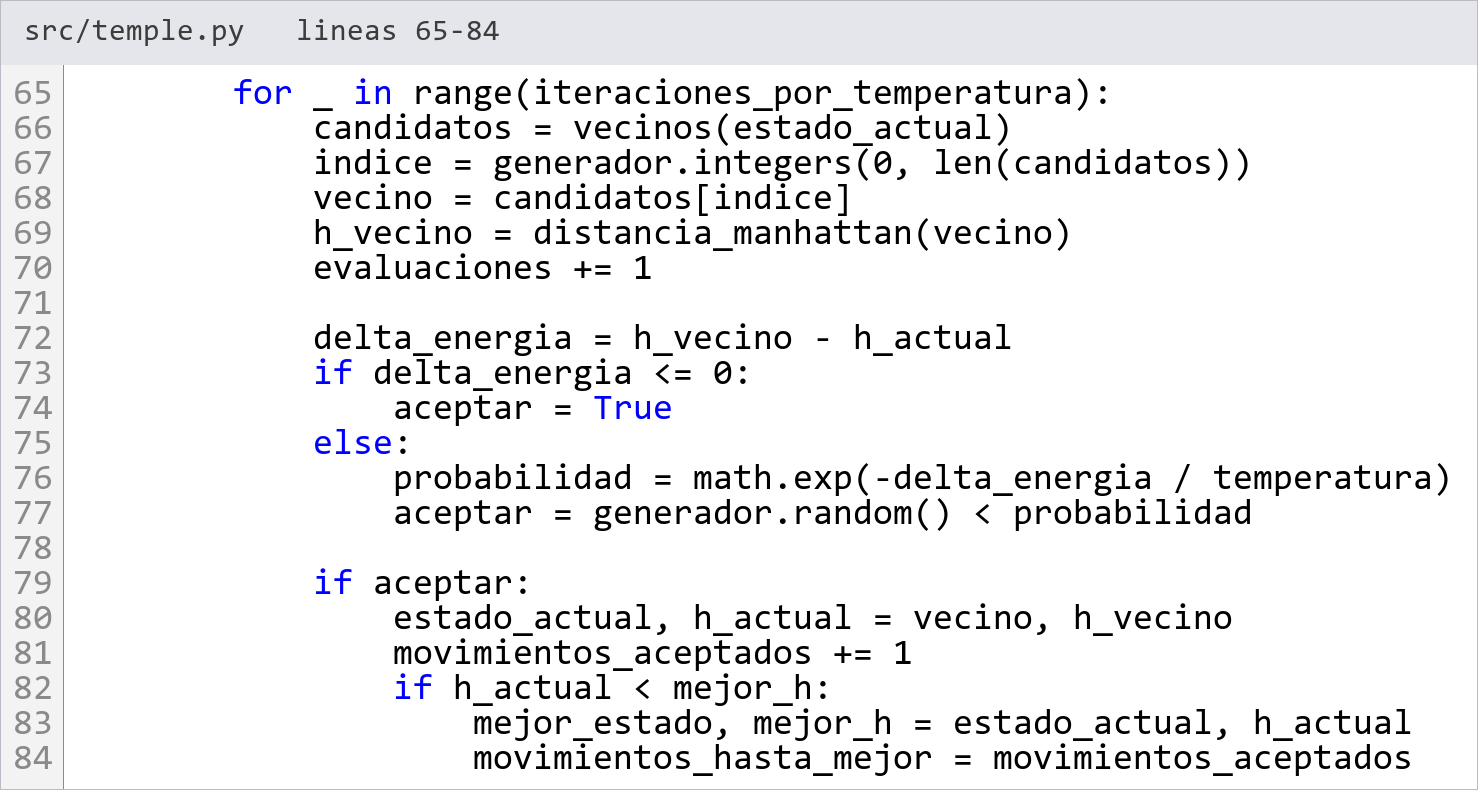
\includegraphics{temple_aceptacion.png}
    \caption{Una iteración de temple simulado: criterio de aceptación
    de Metropolis. Fuente: elaboración propia
    (\nolinkurl{src/temple.py}).}
    \label{fig:codigo_temple}
\end{figure}

% ====================================================================
\section{Metodología}

\subsection{Conjunto de pruebas}

Se generaron 30 tableros resolubles con semilla fija (42), aplicando el
criterio de paridad de inversiones. Su $h$ inicial promedio es 13.97
(entre 6 y 20), y su solución óptima promedio es de 22.5 movimientos
(entre 16 y 28), calculada con la búsqueda en anchura descrita en el
marco teórico.

\subsection{Métricas}

\begin{itemize}
    \item \textbf{Tasa de éxito}: porcentaje de tableros resueltos
    ($h = 0$). Se calcula por separado en cada semilla, sobre los 30
    tableros, y se reporta el promedio, la desviación estándar, el
    mínimo y el máximo entre las 10 semillas.
    \item \textbf{$h$ final}: valor de $h$ del mejor estado encontrado.
    \item \textbf{Evaluaciones}: número de llamadas a $h(s)$, con el
    mismo criterio en todos los algoritmos (una por cada estado
    evaluado, incluido el inicial). Es la medida de costo
    computacional.
    \item \textbf{Porcentaje de corridas truncadas}: corridas que
    agotaron el presupuesto de evaluaciones sin llegar a $h = 0$, con
    el mismo criterio para temple y para reinicios.
    \item \textbf{Longitud de la solución}: número de movimientos de la
    secuencia que lleva del tablero asignado a la meta, solo en
    corridas resueltas. En temple son los movimientos aceptados hasta
    llegar a $h = 0$; en reinicios, los movimientos de la caminata del
    intento exitoso más los pasos del ascenso. No se eliminan los
    ciclos (movimientos que se deshacen).
    \item \textbf{Razón sobre la óptima}: longitud de la solución
    dividida por la longitud óptima del mismo tablero.
\end{itemize}

\subsection{Decisiones de diseño}

\subsubsection{Varias semillas por tablero}

Todo lo aleatorio (estocástico, reinicios y temple, incluidos los
barridos) se repitió con 10 semillas por tablero, es decir, 300
corridas por configuración. Steepest es determinista y corre una vez
por tablero. La decisión surgió de una prueba: la misma configuración
de temple ($T_0 = 10$, $\alpha = 0.97$), corrida una sola vez sobre los
30 tableros con 8 semillas distintas, dio tasas de éxito de 53.3\%,
66.7\%, 66.7\%, 70.0\%, 70.0\%, 73.3\%, 76.7\% y 90.0\%. Un rango de 37
puntos para una misma configuración es mayor que la mayoría de las
diferencias entre configuraciones: una sola corrida no alcanza para
comparar algoritmos estocásticos.

Cada corrida usa su propio generador de números aleatorios, con una
semilla derivada de la configuración, la semilla y el tablero. En
temple, la semilla depende de $(T_0, \alpha)$ y no del experimento que
la corre, así que una misma configuración da exactamente los mismos
números en el barrido y en la tabla principal.

\subsubsection{Presupuesto compartido de evaluaciones}

Para comparar con el mismo costo computacional, todas las
configuraciones aleatorias de la tabla principal (reinicios, temple de
la actividad y temple mejor) y todos los barridos usan el mismo tope de
evaluaciones: \textbf{9823}. Es el promedio de evaluaciones que gasta
temple con la configuración de la actividad ($T_0 = 10$,
$\alpha = 0.97$) cuando corre hasta su parada natural. Reinicios
necesita un tope porque no tiene criterio de parada propio, y el temple
lo necesita para que una configuración no gane solo por enfriar más
lento y gastar más evaluaciones.

Para que el porcentaje de corridas truncadas sea comparable entre
algoritmos, temple y reinicios usan la misma función para decidir si
una corrida fue truncada (Figura \ref{fig:codigo_truncada}). Una
corrida queda truncada solo si tenía presupuesto, no llegó a $h = 0$ y
gastó todo el presupuesto (líneas 201 a 203). Una corrida que termina
por su parada natural (temple que llega a $T_{\min}$) o que resuelve el
tablero justo al agotar el presupuesto no cuenta como truncada.

\begin{figure}[H]
    \centering
    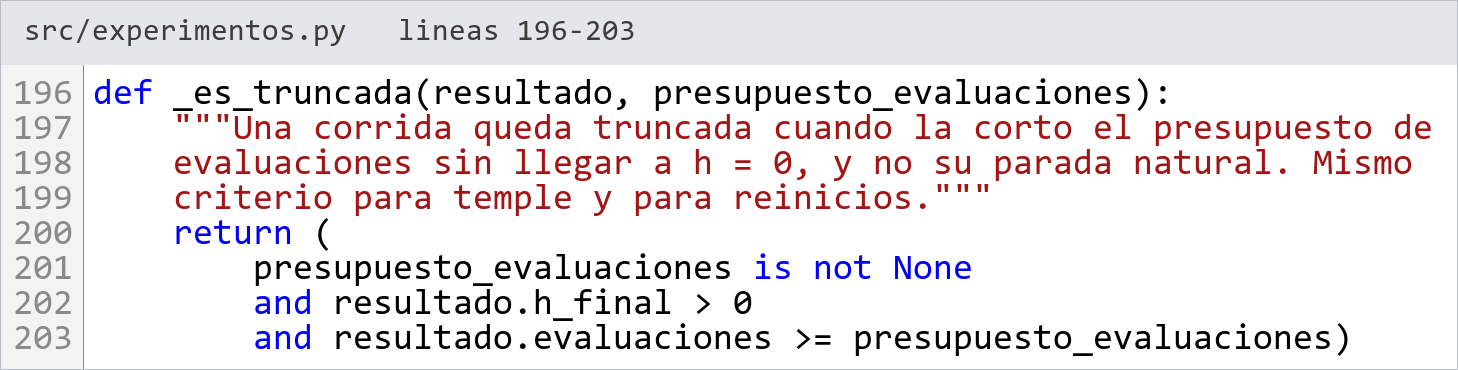
\includegraphics{es_truncada.png}
    \caption{Criterio de truncado compartido por temple y reinicios.
    Fuente: elaboración propia (\nolinkurl{src/experimentos.py}).}
    \label{fig:codigo_truncada}
\end{figure}

\subsubsection{Parámetros fijos de temple}

Se usaron $L = 100$ iteraciones por nivel y $T_{\min} = 0.05$. Con
$T = 0.05$, aceptar un empeoramiento tiene probabilidad $e^{-20}$: el
temple ya está congelado. Se probó $T_{\min} = 0.01$ (el valor de un
cuaderno exploratorio previo): temple de la actividad sin tope dio
exactamente la misma tasa de éxito (70.3\%), pero gastó 11\,395
evaluaciones en lugar de 9823, porque solo alarga la cola del
enfriamiento. Bajarlo habría inflado el presupuesto compartido sin
cambiar el resultado.

\subsubsection{Barrido de \texorpdfstring{$T_0$}{T0} y \texorpdfstring{$\alpha$}{alpha}}

La mejor configuración de temple se eligió con un barrido sobre la
grilla
\begin{equation*}
    T_0 \in \{0.5, 1, 2, 5, 10, 20, 40\}, \qquad
    \alpha \in \{0.90, 0.95, 0.97, 0.99, 0.995, 0.998\}
\end{equation*}
(42 combinaciones), sobre los 30 tableros, con 10 semillas y el presupuesto
compartido. Se eligió la de mayor tasa de éxito promedio y, en caso de
empate, la de menos evaluaciones. Una primera versión del barrido usaba
10 tableros y una grilla sin $T_0$ bajos ni $\alpha$ altos; se amplió
porque la muestra chica elegía configuraciones que después rendían
peor en el conjunto completo, y porque la zona de $T_0$ bajo y
$\alpha$ alto era justo donde el cuaderno exploratorio había encontrado
buenos resultados.

Las combinaciones que enfrían lento no alcanzan a llegar a $T_{\min}$
dentro del presupuesto y quedan truncadas. Se dejaron competir así a
propósito: el barrido responde qué configuración rinde más con el mismo
costo, y enfriar lento es justamente gastar más evaluaciones.

\subsubsection{Reinicios por perturbación y elección de \texorpdfstring{$K$}{K}}

La primera implementación de reinicios partía de tableros resolubles
generados al azar, sin relación con el tablero asignado. Llegó a
99.0\% de éxito, pero ninguno de los 300 intentos exitosos partía del
tablero asignado: resolvía otros tableros, no el que se le pedía, y no
producía una secuencia de movimientos que resolviera el tablero dado.
Por eso se reemplazó por \textbf{reinicios por perturbación}: el primer
intento es un ascenso más pronunciado desde el tablero asignado; si
queda en un mínimo local, cada reinicio hace una caminata aleatoria de
$K$ movimientos legales partiendo siempre del tablero asignado y
vuelve a aplicar el ascenso. Así, todo intento exitoso (caminata más
ascenso) es una solución real del tablero asignado.

La caminata (Figura \ref{fig:codigo_caminata}) aplica $K$ movimientos
legales, cada uno elegido al azar entre los vecinos del estado actual
(líneas 79 a 81). Como usa la misma función \texttt{vecinos} que el
resto de los algoritmos, el tablero que produce siempre es alcanzable
desde el de partida. La caminata no calcula $h$, así que sus
movimientos no cuentan como evaluaciones.

\begin{figure}[H]
    \centering
    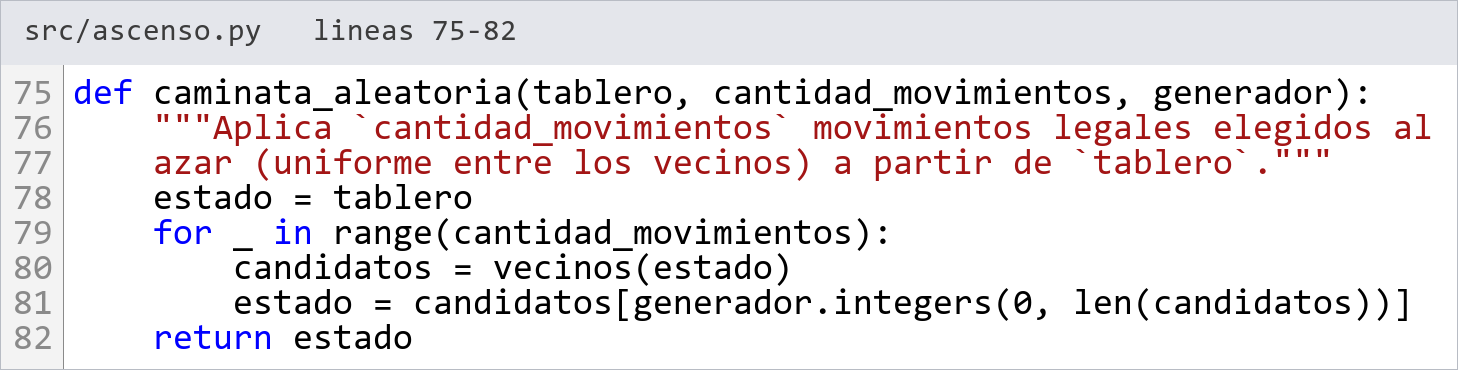
\includegraphics{caminata_aleatoria.png}
    \caption{Caminata aleatoria de $K$ movimientos legales usada para
    perturbar el tablero. Fuente: elaboración propia
    (\nolinkurl{src/ascenso.py}).}
    \label{fig:codigo_caminata}
\end{figure}

El bucle principal de reinicios (Figura \ref{fig:codigo_reinicios})
muestra por qué la solución sigue siendo real. En la primera vuelta,
\texttt{tablero} es el tablero asignado, así que el primer intento es
un ascenso directo. Cada reinicio siguiente parte de una caminata que
empieza \emph{siempre} en \texttt{tablero\_inicial} (líneas 135 y 136),
no en el punto de partida del reinicio anterior; si las caminatas se
encadenaran, el algoritmo se alejaría cada vez más del tablero asignado.
Cuando un intento llega a $h = 0$, la solución es la caminata de ese
intento seguida de los pasos del ascenso, y su longitud se registra
como la suma de ambos (línea 132). El costo del punto de partida y del
ascenso se descuenta del presupuesto (líneas 123 y 127).

\begin{figure}[H]
    \centering
    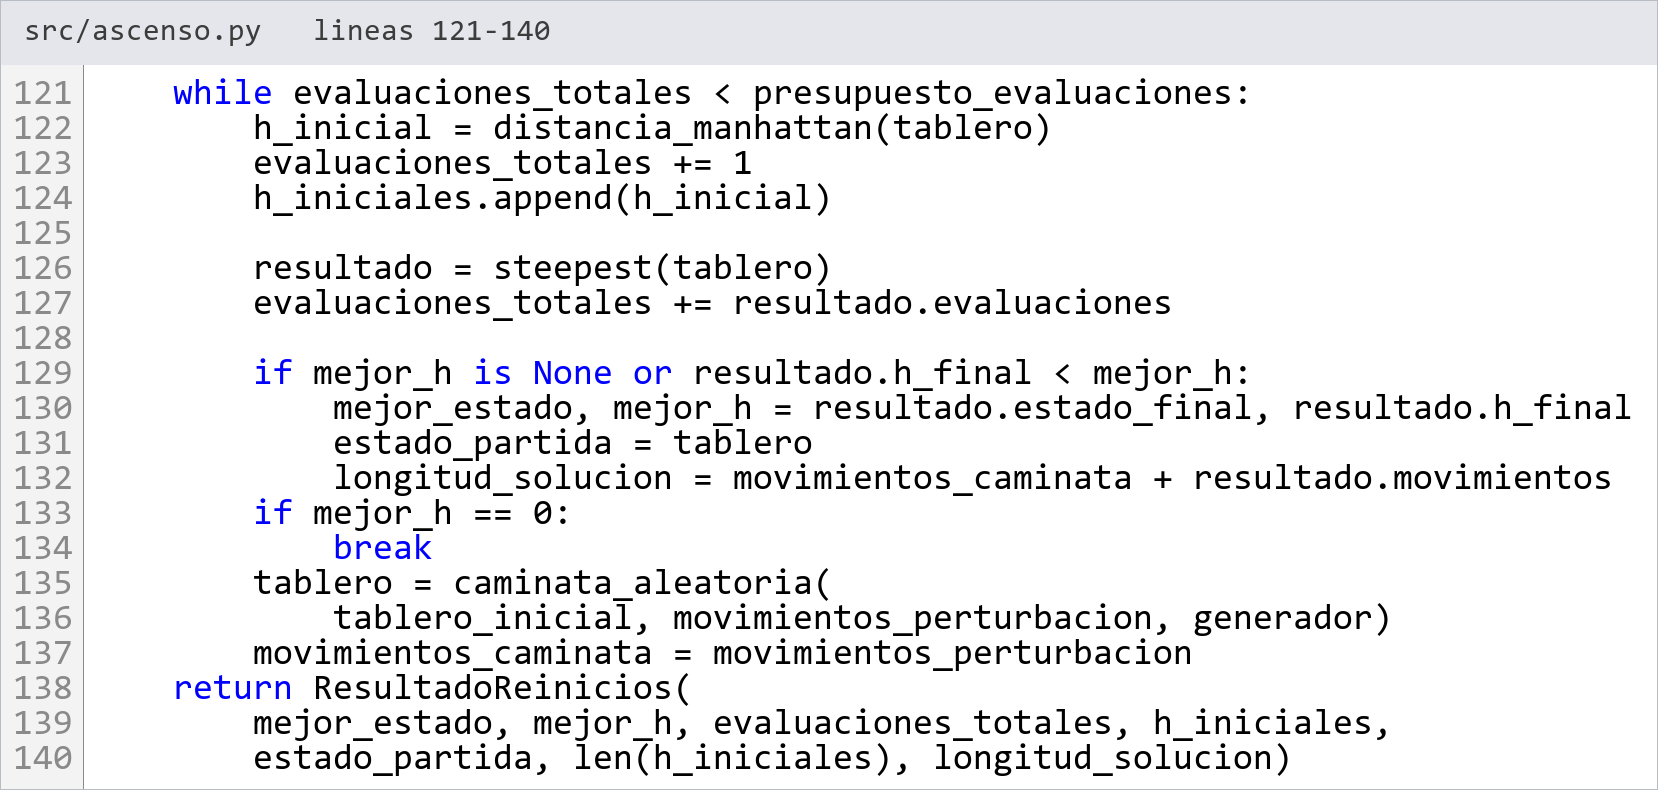
\includegraphics{reinicios_bucle.png}
    \caption{Bucle de reinicios por perturbación: cada reinicio parte
    del tablero asignado. Fuente: elaboración propia
    (\nolinkurl{src/ascenso.py}).}
    \label{fig:codigo_reinicios}
\end{figure}

El largo $K$ de la caminata se fijó en \textbf{$K = 20$} usando el
diámetro del espacio de estados. Con $K < 31$ la caminata sigue siendo
una modificación local del tablero asignado. Con $K \ge 31$ ya tiene
alcance para llegar a cualquier tablero resoluble, y el reinicio se
parece cada vez más a generar un tablero al azar. $K = 20$ es el mayor
valor redondo por debajo de ese umbral. El barrido
$K \in \{10, 20, 50, 100, 200\}$ se reporta aparte como análisis del
efecto de $K$, no como criterio de selección.

En el código, la decisión queda fijada como una constante documentada
y no como un número suelto (Figura \ref{fig:codigo_k}): el comentario
registra el umbral del diámetro y aclara que el barrido de $K$ no
elige el valor principal (líneas 70 a 72). Así, quien lea el código
encuentra la misma justificación que este informe.

\begin{figure}[H]
    \centering
    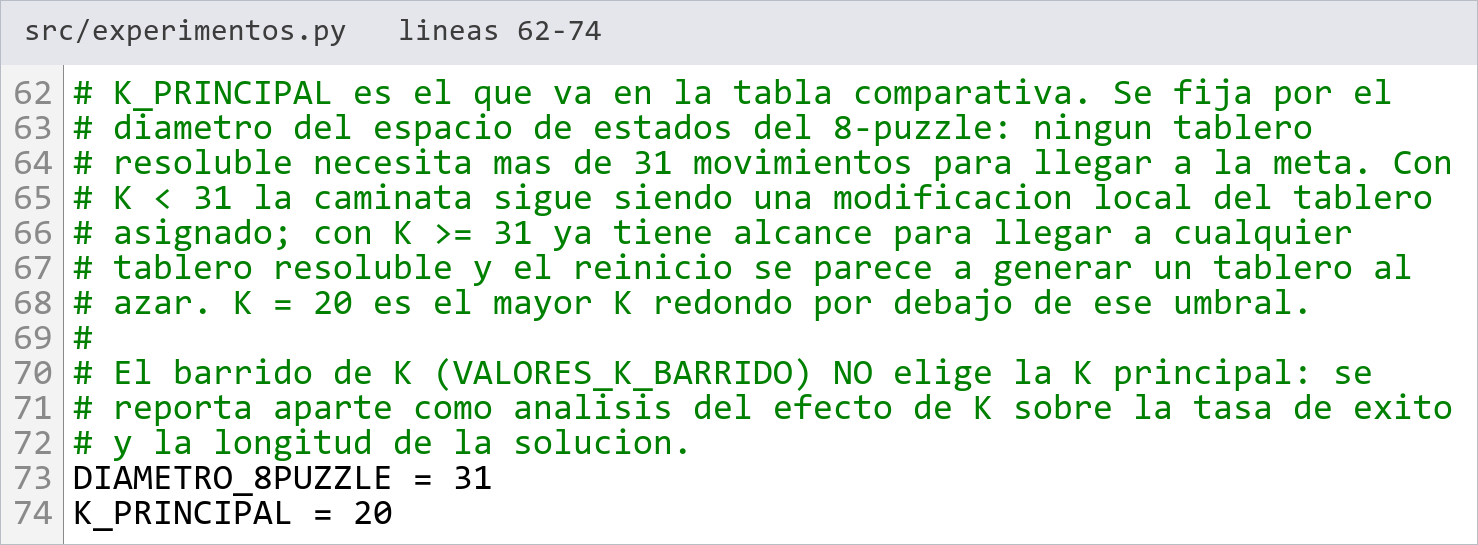
\includegraphics{k_principal.png}
    \caption{Elección de $K$ por el diámetro del espacio de estados.
    Fuente: elaboración propia (\nolinkurl{src/experimentos.py}).}
    \label{fig:codigo_k}
\end{figure}

\subsection{Configuraciones comparadas}

\begin{table}[H]
\centering
\caption{Configuraciones de la tabla principal}
\label{tab:configuraciones}
\begin{tabular}{lp{8.5cm}}
\toprule
\textbf{Configuración} & \textbf{Descripción} \\
\midrule
Steepest & Ascenso más pronunciado desde el tablero asignado. \\
Estocástico & Ascenso estocástico desde el tablero asignado. \\
Reinicios & Reinicios por perturbación con $K = 20$, presupuesto 9823. \\
Temple (actividad) & $T_0 = 10$, $\alpha = 0.97$, presupuesto 9823. \\
Temple (mejor) & $T_0 = 1$, $\alpha = 0.998$ (ganadora del barrido), presupuesto 9823. \\
\bottomrule
\end{tabular}
\end{table}

En todas las configuraciones de temple, $L = 100$ y $T_{\min} = 0.05$.

% ====================================================================
\section{Resultados}

\subsection{Tabla principal}

\begin{table}[H]
\centering
\caption{Resultados con el mismo presupuesto (30 tableros, 10 semillas)}
\label{tab:principal}
\small
\begin{tabular}{lrrrrrr}
\toprule
\textbf{Configuración} & \textbf{Éxito (\%)} & \textbf{Desv.} & \textbf{Mín--máx} & \textbf{$h$ final} & \textbf{Evaluac.} & \textbf{Trunc. (\%)} \\
\midrule
Steepest           & 0.0  & 0.00 & 0.0--0.0   & 12.53 & 7.4    & 0.0 \\
Estocástico        & 0.0  & 0.00 & 0.0--0.0   & 12.35 & 7.9    & 0.0 \\
Reinicios ($K=20$) & 32.7 & 5.54 & 26.7--43.3 & 2.92  & 7568.7 & 67.3 \\
Temple (actividad) & 68.0 & 7.02 & 56.7--80.0 & 1.05  & 7563.6 & 32.0 \\
Temple (mejor)     & 96.3 & 4.07 & 86.7--100  & 0.13  & 3074.5 & 3.7 \\
\bottomrule
\end{tabular}
\end{table}

\begin{figure}[H]
    \centering
    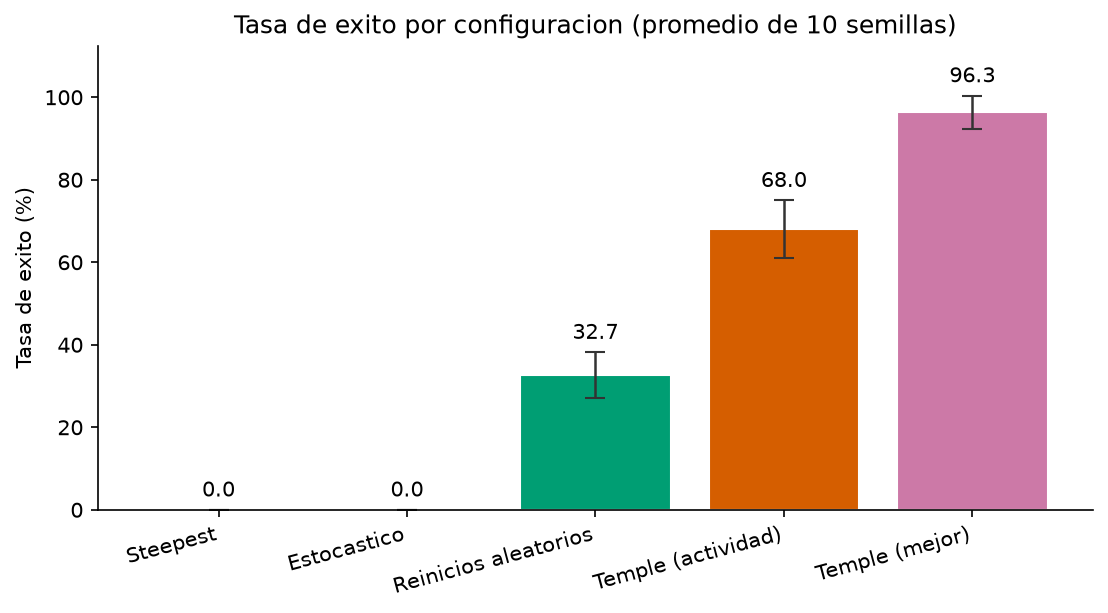
\includegraphics[width=0.85\textwidth]{ascenso_temple_tasa_exito.png}
    \caption{Tasa de éxito promedio por configuración; las barras de
    error son la desviación estándar entre semillas. Fuente:
    elaboración propia.}
    \label{fig:tasa_exito}
\end{figure}

\begin{figure}[H]
    \centering
    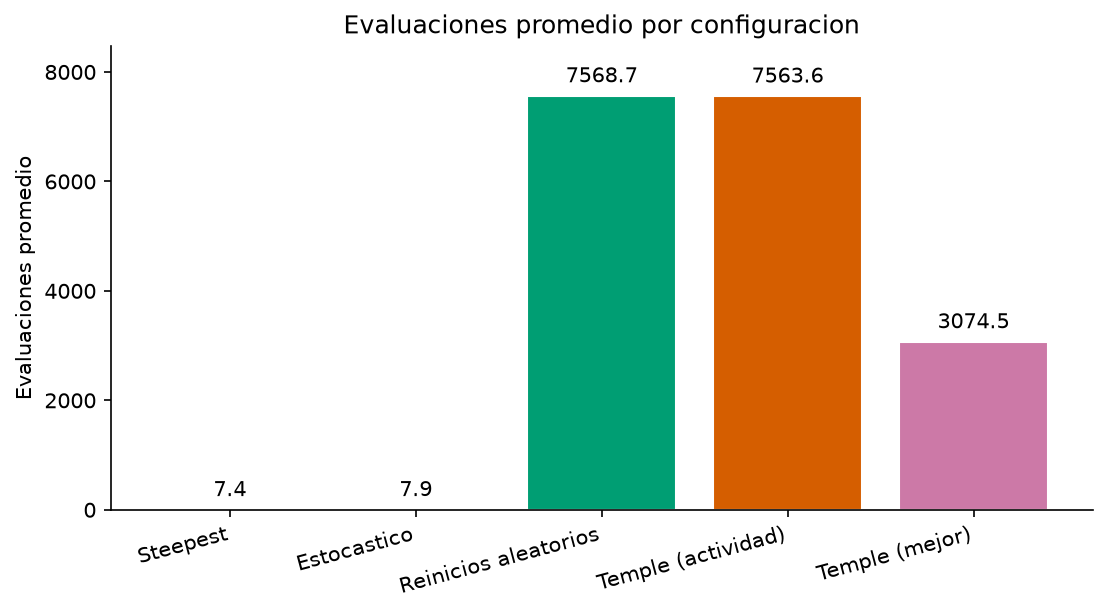
\includegraphics[width=0.85\textwidth]{ascenso_temple_evaluaciones_promedio.png}
    \caption{Evaluaciones promedio de $h$ por configuración. Fuente:
    elaboración propia.}
    \label{fig:evaluaciones}
\end{figure}

\subsection{Longitud de la solución}

\begin{table}[H]
\centering
\caption{Longitud de la solución en las corridas resueltas}
\label{tab:longitud}
\begin{tabular}{lrrrr}
\toprule
\textbf{Configuración} & \textbf{Resueltas} & \textbf{Longitud prom.} & \textbf{Mín--máx} & \textbf{Veces la óptima} \\
\midrule
Reinicios ($K=20$) & 98/300  & 31.5   & 24--40    & 1.6 \\
Temple (actividad) & 204/300 & 5384.9 & 860--6984 & 245.0 \\
Temple (mejor)     & 289/300 & 1473.7 & 51--4756  & 66.9 \\
\bottomrule
\end{tabular}
\end{table}

Steepest y estocástico no resolvieron ningún tablero. La solución
óptima promedio es de 22.5 movimientos en el conjunto completo; en los
tableros que resuelve reinicios es de 19.9, y en los que resuelve
temple mejor, de 22.5. Ninguna configuración encontró nunca la
solución óptima exacta de un tablero.

\begin{figure}[H]
    \centering
    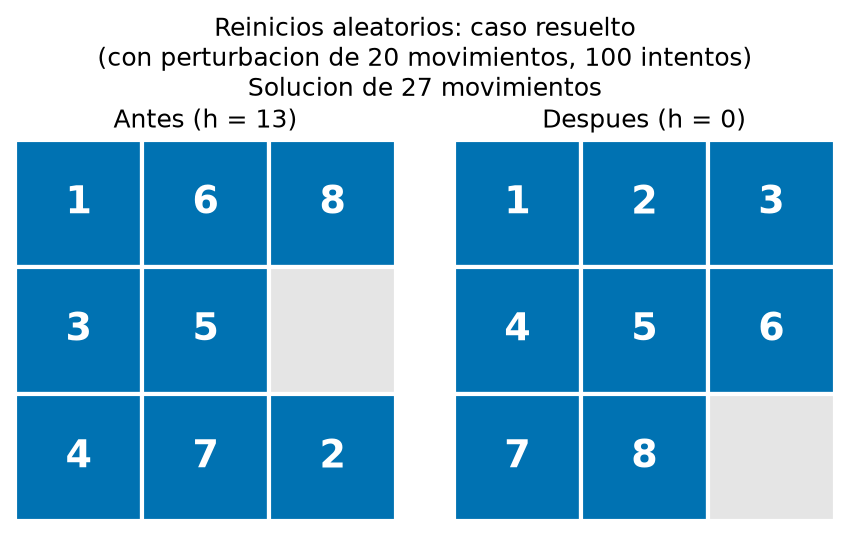
\includegraphics[width=0.49\textwidth]{antes_despues_reinicios.png}
    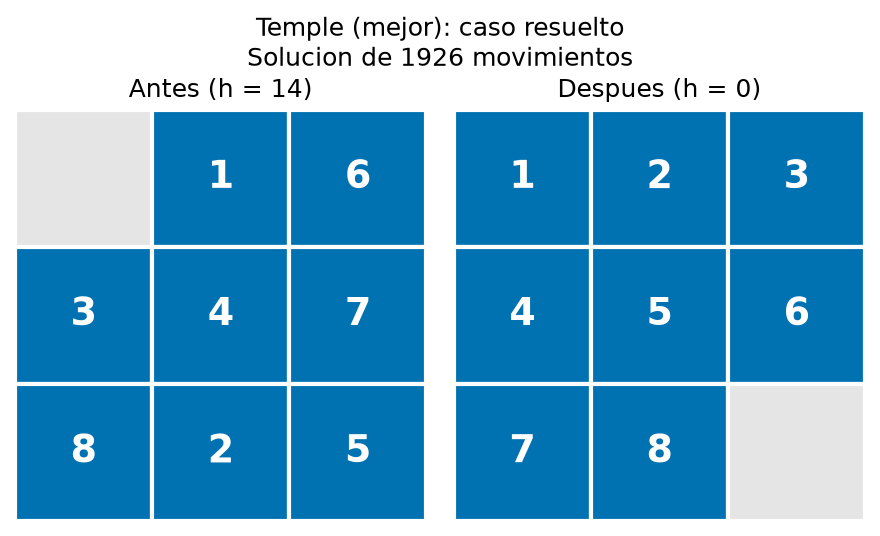
\includegraphics[width=0.49\textwidth]{antes_despues_temple_mejor.png}
    \caption{Casos resueltos por reinicios ($K = 20$) y por temple
    mejor, con la longitud de la solución de cada uno. Fuente:
    elaboración propia.}
    \label{fig:antes_despues}
\end{figure}

\subsection{Ascenso puro y degradación del temple}

\begin{figure}[H]
    \centering
    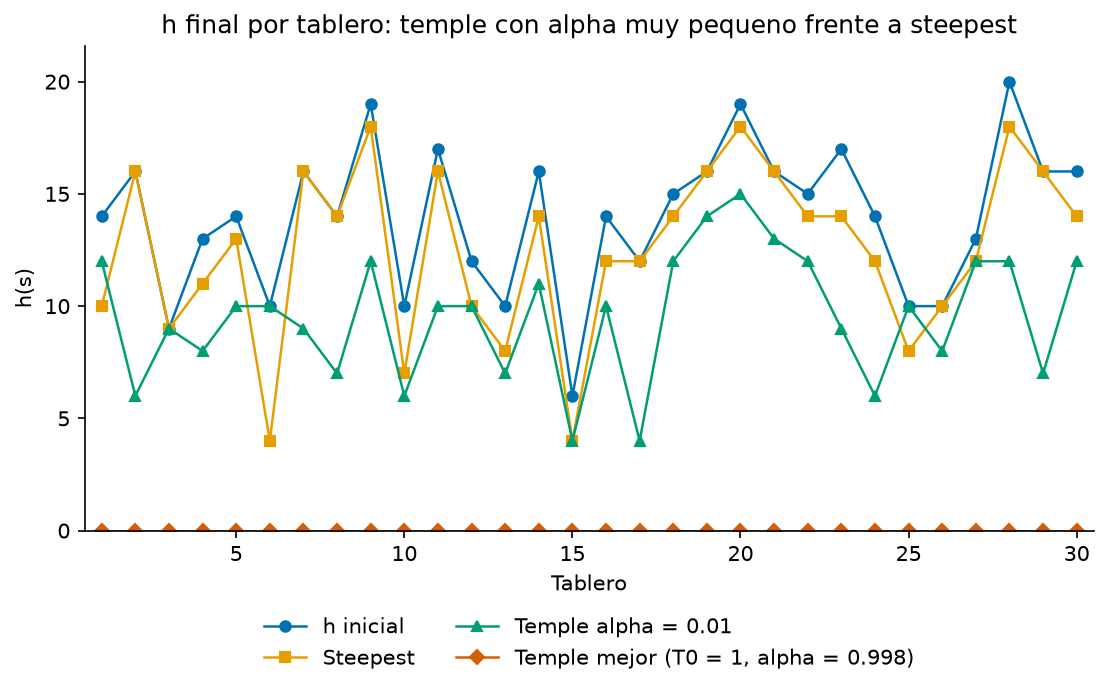
\includegraphics[width=0.85\textwidth]{temple_alpha_pequeno_vs_ascenso.png}
    \caption{$h$ final por tablero: steepest, temple con $\alpha =
    0.01$ (enfriamiento casi inmediato) y temple mejor. Fuente:
    elaboración propia.}
    \label{fig:degradacion}
\end{figure}

Steepest hace en promedio 1.4 movimientos antes de quedar atrapado: la
mayoría de los tableros de prueba ya están en un mínimo local o muy
cerca de uno. Temple con $\alpha = 0.01$ tampoco resolvió ninguno de
los 30 tableros ($h$ final promedio 9.57): después del primer nivel de
temperatura, $T$ ya es tan baja que solo acepta mejoras y se comporta
como un ascenso de colinas.

\subsection{Trazas de temple}

\begin{figure}[H]
    \centering
    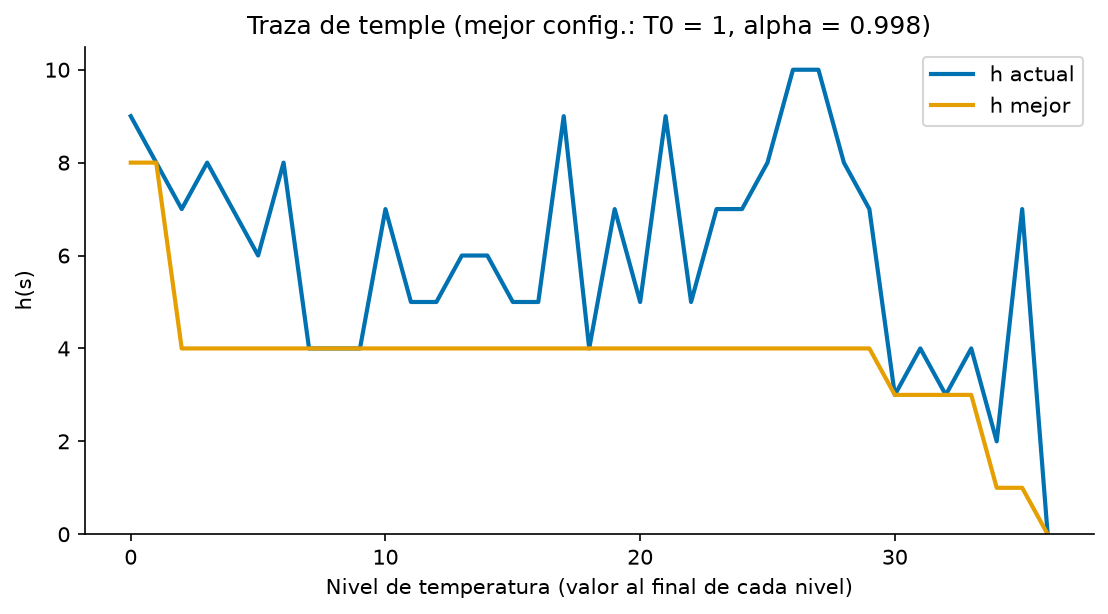
\includegraphics[width=0.85\textwidth]{temple_mejor_traza.png}
    \caption{Evolución de $h$ actual y $h$ mejor en una corrida de
    temple mejor (tablero 1), al final de cada nivel de temperatura.
    Fuente: elaboración propia.}
    \label{fig:traza_mejor}
\end{figure}

\begin{figure}[H]
    \centering
    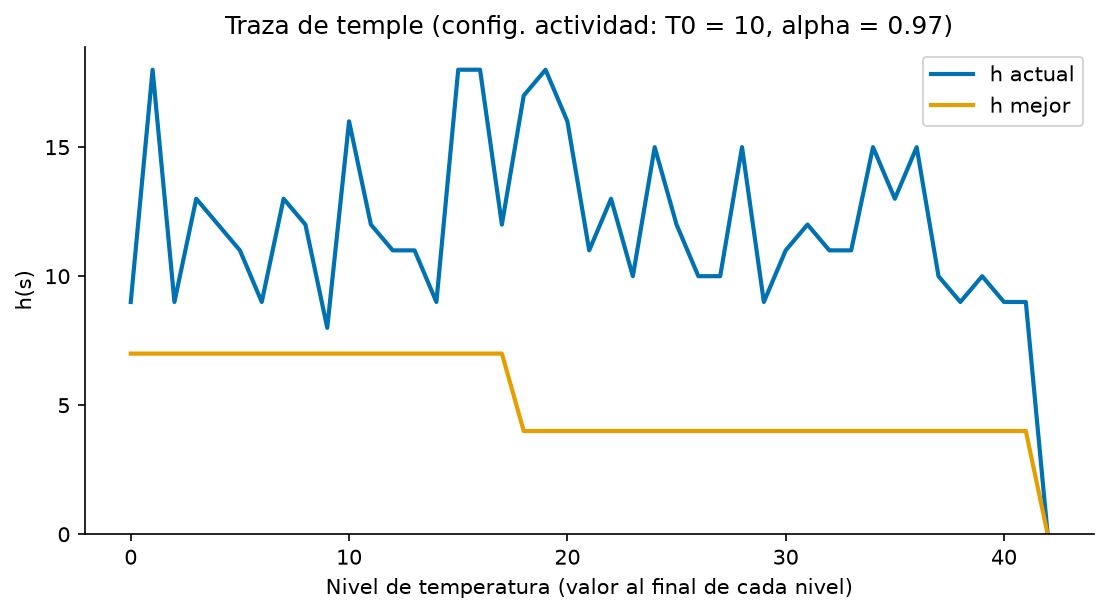
\includegraphics[width=0.85\textwidth]{temple_actividad_traza.png}
    \caption{Evolución de $h$ en una corrida de temple de la actividad
    (tablero 1). Fuente: elaboración propia.}
    \label{fig:traza_actividad}
\end{figure}

\subsection{Barrido de \texorpdfstring{$T_0$}{T0} y \texorpdfstring{$\alpha$}{alpha}}

\begin{table}[H]
\centering
\caption{Las seis mejores combinaciones del barrido $T_0 \times \alpha$}
\label{tab:barrido_temple}
\begin{tabular}{rrrrrr}
\toprule
\textbf{$T_0$} & \textbf{$\alpha$} & \textbf{Éxito (\%)} & \textbf{Desv.} & \textbf{Evaluac.} & \textbf{Trunc. (\%)} \\
\midrule
1 & 0.998 & 96.3 & 4.1 & 3074.5 & 3.7 \\
1 & 0.995 & 93.7 & 5.7 & 3220.1 & 6.3 \\
2 & 0.99  & 90.7 & 2.5 & 4363.0 & 9.3 \\
2 & 0.995 & 87.3 & 5.5 & 4750.5 & 12.7 \\
1 & 0.99  & 78.3 & 8.9 & 3913.2 & 21.7 \\
2 & 0.998 & 77.3 & 8.0 & 5665.2 & 22.7 \\
\bottomrule
\end{tabular}
\end{table}

\begin{figure}[H]
    \centering
    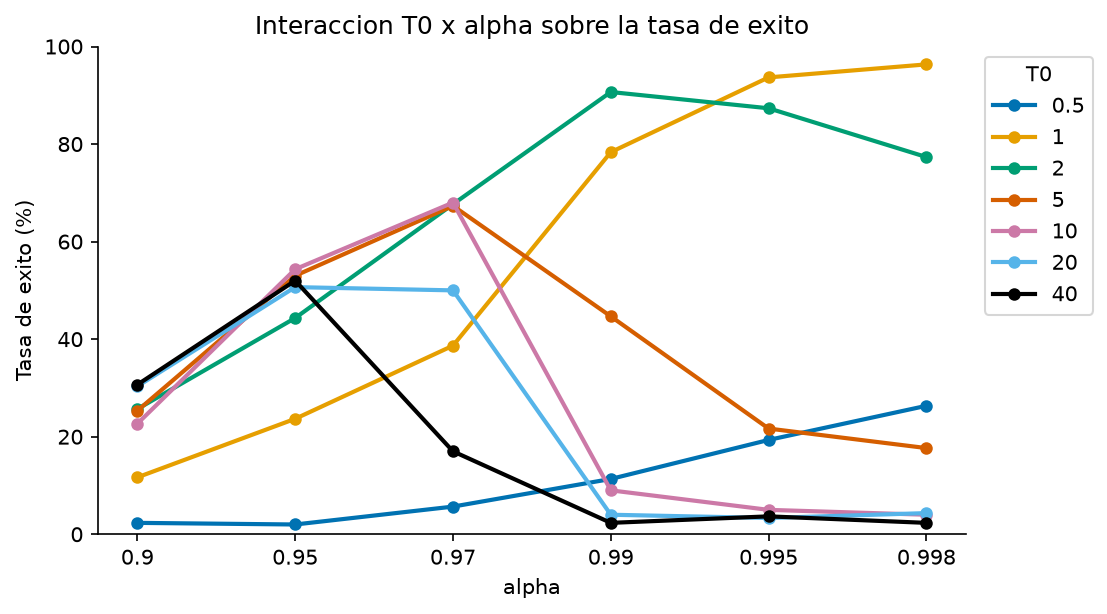
\includegraphics[width=0.85\textwidth]{temple_interaccion_t0_alpha.png}
    \caption{Tasa de éxito para cada combinación de $T_0$ y $\alpha$
    (una curva por $T_0$). Fuente: elaboración propia.}
    \label{fig:interaccion}
\end{figure}

\begin{figure}[H]
    \centering
    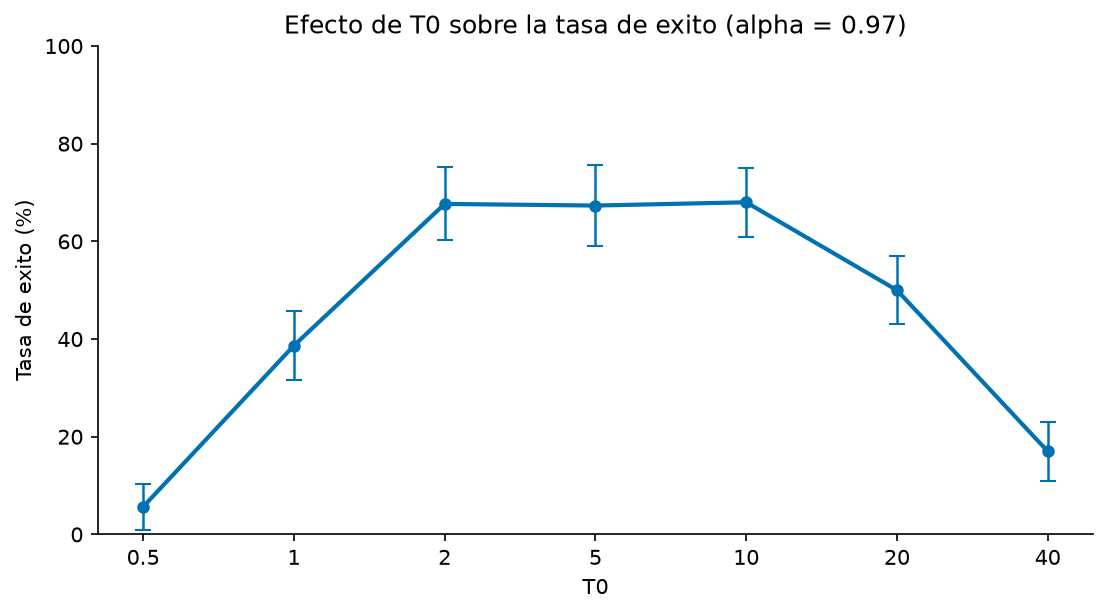
\includegraphics[width=0.49\textwidth]{temple_efecto_t0.png}
    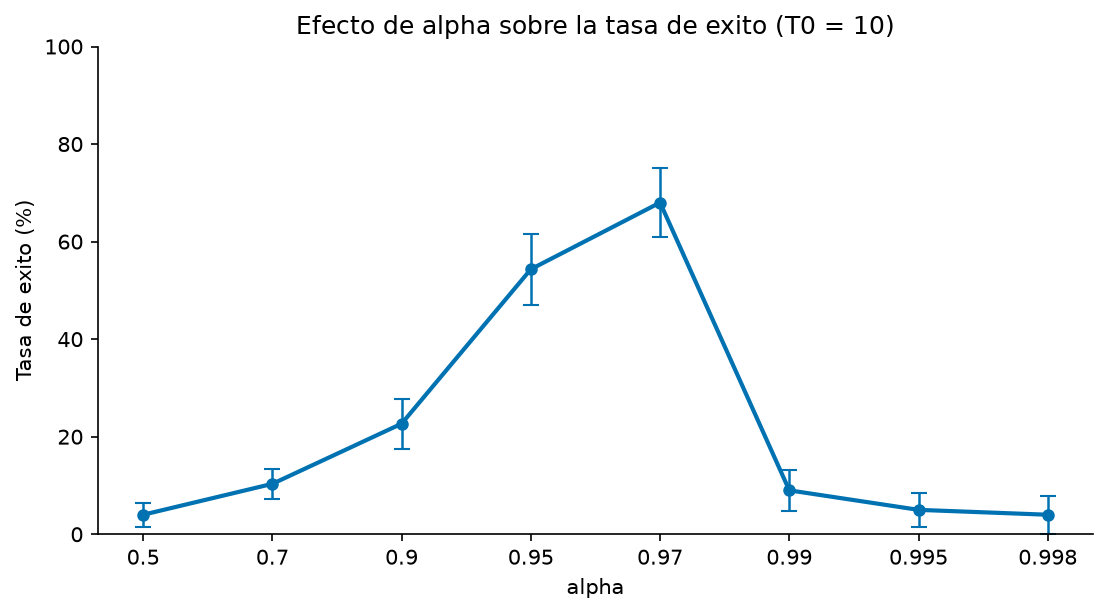
\includegraphics[width=0.49\textwidth]{temple_efecto_alpha.png}
    \caption{Efecto de $T_0$ con $\alpha = 0.97$ (izquierda) y de
    $\alpha$ con $T_0 = 10$ (derecha). Fuente: elaboración propia.}
    \label{fig:efectos}
\end{figure}

\subsection{Barrido de \texorpdfstring{$K$}{K} (análisis aparte)}

\begin{table}[H]
\centering
\caption{Reinicios por perturbación según el largo $K$ de la caminata}
\label{tab:barrido_k}
\begin{tabular}{rrrrrr}
\toprule
\textbf{$K$} & \textbf{Éxito (\%)} & \textbf{Desv.} & \textbf{Evaluac.} & \textbf{Trunc. (\%)} & \textbf{Longitud prom.} \\
\midrule
10  & 10.3 & 1.8 & 9089.0 & 89.7 & 21.2 \\
20  & 32.7 & 5.5 & 7568.7 & 67.3 & 31.5 \\
50  & 80.3 & 5.3 & 4500.6 & 19.7 & 61.5 \\
100 & 95.0 & 3.1 & 2898.4 & 5.0  & 110.9 \\
200 & 97.3 & 2.5 & 2545.8 & 2.7  & 210.9 \\
\bottomrule
\end{tabular}
\end{table}

\begin{figure}[H]
    \centering
    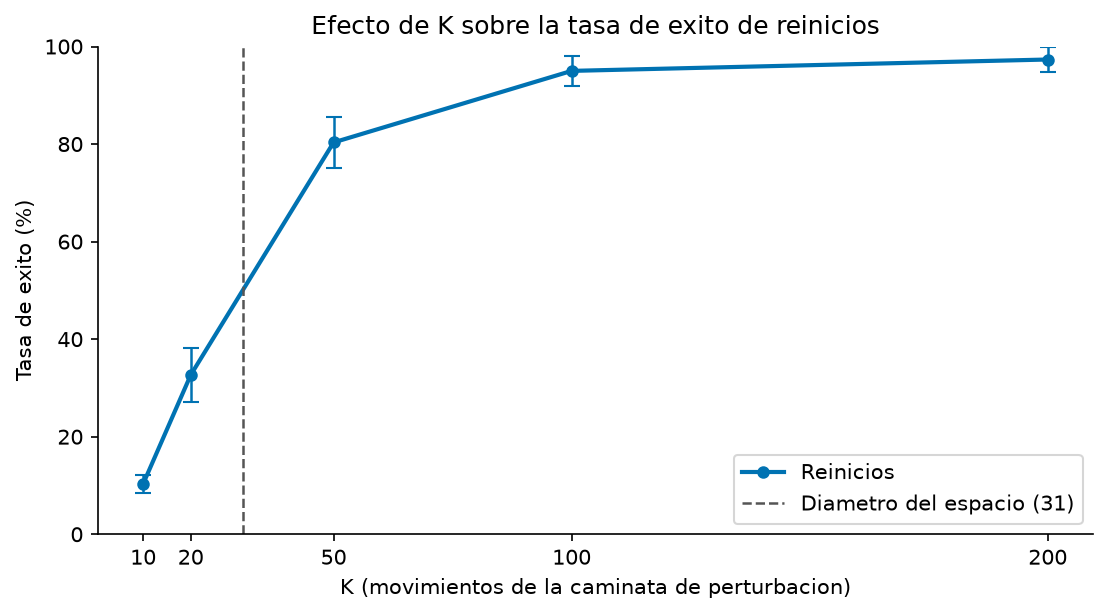
\includegraphics[width=0.85\textwidth]{reinicios_efecto_k.png}
    \caption{Tasa de éxito de reinicios según $K$; la línea punteada
    marca el diámetro del espacio de estados. Fuente: elaboración
    propia.}
    \label{fig:efecto_k}
\end{figure}

\begin{figure}[H]
    \centering
    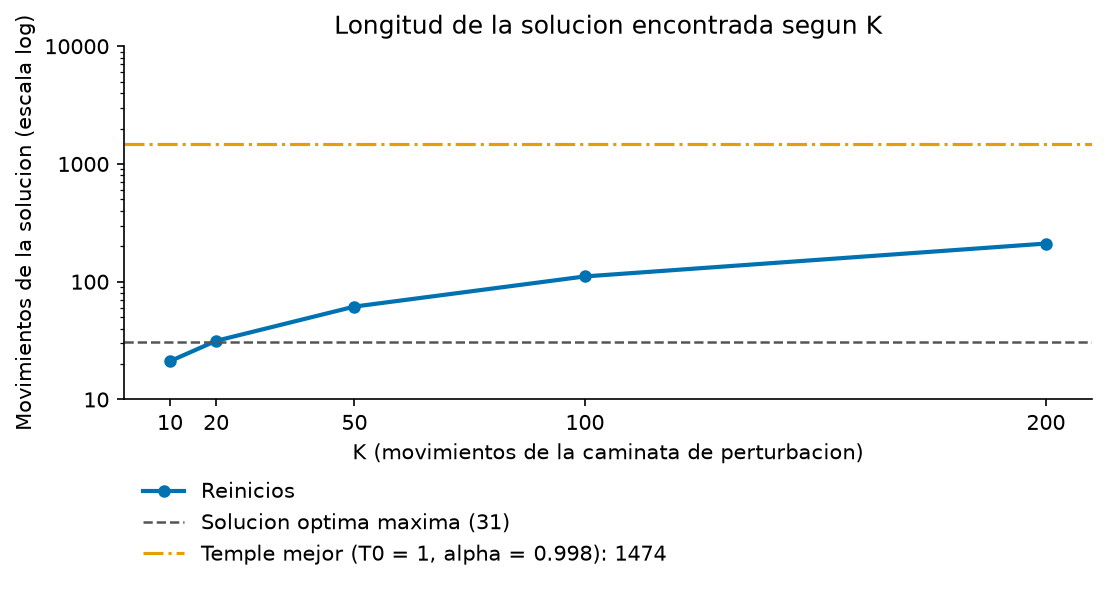
\includegraphics[width=0.85\textwidth]{reinicios_longitud_vs_k.png}
    \caption{Longitud promedio de la solución de reinicios según $K$
    (escala logarítmica), frente a la solución óptima máxima (31) y a
    temple mejor. Fuente: elaboración propia.}
    \label{fig:longitud_k}
\end{figure}

\subsection{Temple sin tope de evaluaciones}

\begin{table}[H]
\centering
\caption{Temple de la actividad con y sin presupuesto (mismas semillas)}
\label{tab:sin_tope}
\begin{tabular}{lrrrr}
\toprule
\textbf{Configuración} & \textbf{Éxito (\%)} & \textbf{Desv.} & \textbf{Evaluac.} & \textbf{Trunc. (\%)} \\
\midrule
Con presupuesto (9823) & 68.0 & 7.02 & 7563.6 & 32.0 \\
Sin tope               & 70.3 & 6.74 & 9822.6 & 0.0 \\
\bottomrule
\end{tabular}
\end{table}

\begin{figure}[H]
    \centering
    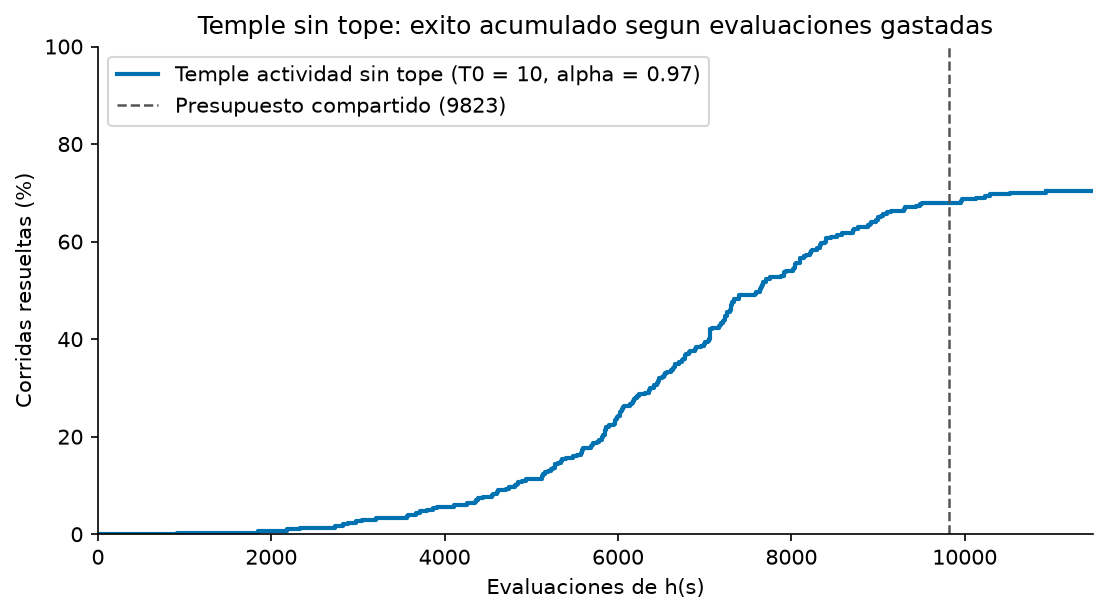
\includegraphics[width=0.85\textwidth]{temple_sin_tope_exito_acumulado.png}
    \caption{Porcentaje de corridas resueltas según las evaluaciones
    gastadas, para temple de la actividad sin tope. Fuente:
    elaboración propia.}
    \label{fig:sin_tope}
\end{figure}

% ====================================================================
\section{Análisis}

\subsection{El 8-puzzle exige tolerar empeoramientos}

Steepest y estocástico no resolvieron ningún tablero (Tabla
\ref{tab:principal}). Steepest hace en promedio 1.4 movimientos y queda
atrapado, con un $h$ final promedio de 12.53 frente a 13.97 inicial.
Como cada movimiento cambia $h$ en $\pm 1$, un ascenso desde un mínimo
local no tiene ninguna salida: todos los vecinos empeoran. Para llegar
a la meta hay que pasar por estados peores. Esto confirma lo que
plantea la teoría: sin un mecanismo para aceptar empeoramientos
temporales, la búsqueda local queda atrapada en los mínimos locales
del paisaje.

La Figura \ref{fig:degradacion} muestra el mismo fenómeno desde el
temple: con $\alpha = 0.01$ la temperatura cae casi de inmediato,
el temple deja de aceptar empeoramientos y, como steepest, no resuelve
ningún tablero. El barrido de $\alpha$ (Figura \ref{fig:efectos}) lo
confirma de forma gradual: con $T_0 = 10$, la tasa de éxito baja a
10.3\% con $\alpha = 0.7$ y a 4.0\% con $\alpha = 0.5$.

\subsection{Los dos mecanismos para aceptar empeoramientos}

Los dos algoritmos que resuelven tableros aceptan empeoramientos de
formas distintas:

\begin{itemize}
    \item \textbf{Temple}: acepta empeoramientos uno a uno, con
    probabilidad $e^{-1/T}$, durante toda la búsqueda y de forma cada
    vez más selectiva.
    \item \textbf{Reinicios por perturbación}: acepta un bloque de $K$
    movimientos aleatorios de golpe (la caminata, que empeora o mejora
    $h$ a ciegas) y después solo acepta mejoras (el ascenso).
\end{itemize}

Con el mismo presupuesto de 9823 evaluaciones y $K = 20$, temple mejor
resuelve el 96.3\% de los tableros gastando en promedio 3074.5
evaluaciones, mientras que reinicios resuelve el 32.7\% gastando
7568.7. Temple supera a reinicios en tasa de éxito y en costo. La
diferencia entre las dos tasas (63.7 puntos) es mucho mayor que su
variabilidad entre semillas (desviaciones de 4.07 y 5.54).

\subsection{La calibración decide el resultado}

Ninguno de los dos algoritmos funciona bien con cualquier parámetro.
En temple, la tasa de éxito va de 2.0\% a 96.3\% según $T_0$ y $\alpha$
(Figura \ref{fig:interaccion}). Las mejores combinaciones tienen $T_0$
bajo (1 o 2) y $\alpha$ alto (0.99 a 0.998): una temperatura baja pero
sostenida, en la que se acepta entre un tercio y dos tercios de los
empeoramientos, funciona mejor que empezar muy caliente. Con $T_0$ alto
(20 o 40) y $\alpha$ alto, el temple pasa casi todo el presupuesto en
modo de paseo aleatorio y se trunca antes de enfriarse: con $T_0 = 40$
y $\alpha = 0.998$ se truncan el 97.7\% de las corridas.

La configuración de la actividad ($T_0 = 10$, $\alpha = 0.97$) queda en
68.0\%. Sin tope de evaluaciones sube solo a 70.3\% (Tabla
\ref{tab:sin_tope}): su límite no es el presupuesto, sino el
enfriamiento. Aun sin límite de costo, esta configuración gasta 9823
evaluaciones en promedio, más que reinicios con $K = 20$ (7568.7). Como
referencia, la configuración del cuaderno exploratorio ($T_0 = 1$,
$\alpha = 0.995$, $T_{\min} = 0.01$), corrida sin tope, llegó a 95.3\%
con 7132 evaluaciones.

En reinicios, $K$ cumple un papel parecido al de $T_0$ y $\alpha$
(Tabla \ref{tab:barrido_k}): con $K = 10$ la caminata casi nunca saca
al ascenso de la cuenca del mínimo local (10.3\%), y la tasa de éxito
crece con $K$ hasta 97.3\% con $K = 200$. A partir de $K = 100$,
reinicios alcanza o supera a temple mejor en tasa de éxito y gasta
menos evaluaciones.

\subsection{Por qué \texorpdfstring{$K$}{K} grande no es una perturbación local}

Con $K$ por encima del diámetro (31), la caminata ya puede llegar a
cualquier tablero resoluble, y el reinicio se acerca a lo que hacía la
primera implementación: generar tableros prácticamente al azar hasta
dar con uno desde el que el ascenso llega a la meta. Esa versión
llegaba a 99.0\% sin resolver nunca el tablero pedido. Con $K = 200$ el
algoritmo ya no aprovecha la estructura del tablero asignado: es fuerza
bruta con forma de búsqueda local.

La longitud de la solución lo refleja: crece casi linealmente con $K$
(Figura \ref{fig:longitud_k}), de 31.5 movimientos con $K = 20$ a 61.5
con $K = 50$, 110.9 con $K = 100$ y 210.9 con $K = 200$, frente a una
solución óptima promedio de 22.5. Casi toda la solución es la caminata
aleatoria.

Este argumento, sin embargo, no favorece a temple en calidad de
solución: las soluciones de temple mejor (1473.7 movimientos en
promedio) son unas siete veces más largas que las de reinicios con
$K = 200$. La justificación de $K = 20$ se apoya en el diámetro, es
decir, en que la perturbación siga siendo local, y no en la longitud de
la solución.

\subsection{Tasa de éxito frente a calidad de la solución}

La comparación entre temple y reinicios con $K = 20$ tiene dos caras:

\begin{itemize}
    \item \textbf{Temple gana en tasa de éxito y en costo}: 96.3\%
    contra 32.7\% de éxito, con 3074.5 evaluaciones promedio contra
    7568.7.
    \item \textbf{Reinicios gana ampliamente en longitud de la
    solución}: 31.5 movimientos en promedio (1.6 veces la óptima)
    contra 1473.7 de temple mejor (66.9 veces la óptima) y 5384.9 de
    temple de la actividad (245 veces la óptima).
\end{itemize}

La diferencia se explica por el mecanismo de cada algoritmo. El temple
no tiene memoria de los estados visitados y, con $T$ cerca de 1, acepta
alrededor del 37\% de los movimientos que empeoran $h$. Por eso
zigzaguea: acepta movimientos que deshacen el progreso anterior,
vuelve a estados ya visitados y recorre miles de movimientos antes de
llegar a la meta (Figura \ref{fig:traza_mejor}). En cambio, el ascenso
más pronunciado dentro de reinicios nunca retrocede: cada paso baja $h$
en exactamente 1, así que desde el punto de partida llega a la meta en
a lo sumo $h$ pasos. La solución de reinicios es la caminata de $K$
movimientos más un ascenso corto, lo que da caminos cortos por diseño
cuando el ascenso encuentra una cuenca favorable.

Hay dos matices. Primero, la longitud de temple incluye todos los
ciclos; eliminar los movimientos que se deshacen acortaría sus
soluciones, pero eso no se midió en este trabajo. Segundo, reinicios
resuelve sobre todo los tableros más fáciles (óptima promedio de 19.9
en sus tableros resueltos, frente a 22.5 en los de temple), lo que
también favorece su longitud promedio. Aun con esos matices, la
diferencia es de unas 47 veces (casi dos órdenes de magnitud) y no
cambia la conclusión.

% ====================================================================
\section{Conclusiones}

\begin{enumerate}
    \item \textbf{El ascenso de colinas puro no resuelve el 8-puzzle}.
    Steepest y estocástico dan 0\% de éxito, y temple con enfriamiento
    casi inmediato ($\alpha = 0.01$) también. Resolver el 8-puzzle con
    búsqueda local exige tolerar empeoramientos temporales de $h(s)$,
    como plantea la teoría.

    \item \textbf{Temple simulado es superior para encontrar una
    solución}. Con el mismo presupuesto, temple mejor ($T_0 = 1$,
    $\alpha = 0.998$) resuelve el 96.3\% de los tableros con 3074.5
    evaluaciones promedio, frente a 32.7\% y 7568.7 evaluaciones de
    reinicios con una perturbación local ($K = 20$).

    \item \textbf{Pero la solución que entrega temple es mucho menos
    eficiente en número de movimientos}: 1473.7 movimientos en
    promedio, 66.9 veces la solución óptima, porque zigzaguea sin
    memoria de los estados visitados. Reinicios con perturbación
    acotada al diámetro del problema encuentra soluciones cercanas al
    óptimo cuando tiene éxito (31.5 movimientos, 1.6 veces la óptima),
    aunque con menor tasa de éxito y mayor costo en evaluaciones.

    \item \textbf{La calibración es tan importante como el algoritmo}.
    Temple va de 2.0\% a 96.3\% según $T_0$ y $\alpha$, y reinicios de
    10.3\% a 97.3\% según $K$. Reinicios solo alcanza a temple en tasa
    de éxito con $K \ge 100$, es decir, cuando la perturbación supera
    el diámetro del espacio de estados y el reinicio deja de ser una
    búsqueda local.

    \item \textbf{Comparar algoritmos estocásticos exige varias
    corridas}. Una misma configuración de temple varió entre 53.3\% y
    90.0\% según la semilla. Sin repetir con varias semillas y sin un
    presupuesto común de evaluaciones, la comparación depende del azar
    y de cuánto cómputo recibe cada algoritmo.
\end{enumerate}

En síntesis, la respuesta depende de la pregunta. Si la pregunta es
qué algoritmo encuentra una solución con mayor probabilidad y menor
costo computacional dentro de una búsqueda local genuina, la respuesta
es temple simulado. Si la pregunta es qué algoritmo entrega una mejor
solución (una secuencia de movimientos más corta), la respuesta es
reinicios con perturbación acotada, en los tableros que logra resolver.

% ====================================================================
\newpage
\section*{Referencias}
\addcontentsline{toc}{section}{Referencias}

\begin{thebibliography}{99}

\bibitem{johnson1879}
Johnson, W. W. y Story, W. E. (1879). Notes on the ``15'' puzzle.
\textit{American Journal of Mathematics, 2}(4), 397--404.
\url{https://doi.org/10.2307/2369492}

\bibitem{kirkpatrick1983}
Kirkpatrick, S., Gelatt, C. D. y Vecchi, M. P. (1983). Optimization by
simulated annealing. \textit{Science, 220}(4598), 671--680.
\url{https://doi.org/10.1126/science.220.4598.671}

\bibitem{metropolis1953}
Metropolis, N., Rosenbluth, A. W., Rosenbluth, M. N., Teller, A. H. y
Teller, E. (1953). Equation of state calculations by fast computing
machines. \textit{The Journal of Chemical Physics, 21}(6), 1087--1092.
\url{https://doi.org/10.1063/1.1699114}

\bibitem{reinefeld1993}
Reinefeld, A. (1993). Complete solution of the eight-puzzle and the
benefit of node ordering in IDA*. En \textit{Proceedings of the 13th
International Joint Conference on Artificial Intelligence (IJCAI)}
(pp. 248--253).

\bibitem{russell2021}
Russell, S. y Norvig, P. (2021). \textit{Artificial Intelligence: A
Modern Approach} (4.\textsuperscript{a} ed.). Pearson.

\end{thebibliography}

\end{document}
